\chapter{L'énergie dans les systèmes informatiques}
\label{chap3}

\epigraph{<< With out passion you don't have energy, with out energy you have nothing. >>}{--- \textup{Donald Trump}}

\NoChapterPrefix \NoChapterNumberInRef {\hypersetup{linkcolor=black} \minitoc}

%% numérotation des figures, des tables et des équations préfixé par le numéro de chapitre
\makeatletter
\renewcommand{\thefigure}{\ifnum \c@section>\z@ \thechapter.\fi
 \@arabic\c@figure}
\@addtoreset{figure}{chapter}
\makeatother

\makeatletter
\renewcommand{\thetable}{\ifnum \c@section>\z@ \thechapter.\fi
 \@arabic\c@table}
\@addtoreset{table}{chapter}
\makeatother

\makeatletter
\renewcommand{\theequation}{\ifnum \c@section>\z@ \thechapter.\fi
 \@arabic\c@equation}
\@addtoreset{equation}{chapter}
\makeatother
%%-----------------------------------------------------------------
%% Résumé
%%-----------------------------------------------------------------


%laisser une page ou deux pages vides, telle est la question !
%\EmptyNewPage
\newpage

%********************************************************************************
%********************************************************************************
\section{Introduction}
% \section{Conception des modèles de coût}
% \subsection{Définition et évolution}
% \subsection{Conception des modèles de coût}
% \subsubsection{Identification des paramètres et des formules}
% \subsubsection{Calibration et apprentissage automatique}
% \subsubsection{Évaluation (mesure d'énergie : niveau système, niveau composant)}
La demande croissante de traitement de l'information a entraîné la demande de systèmes de gestion de données plus économiques, plus rapides et plus vastes. En le même temps, une part importante et croissante du coût total de propriété de ces systèmes sont l'énergie et le refroidissement. Ces dernières années, l'augmentation des coûts de l'énergie est devenue l'une des questions cruciales dans les centres de données. La nouvelle approche qui s'oriente vers les technologies de préservation de l'énergie a vu l'apparition et l'émergence des concepts tels que les systèmes éco-énergétiques. Par conséquent, l'objectif des concepteurs du système informatique est allé vers la puissance électrique et l'efficacité énergétique. 

Toutefois, pour résoudre à la fois le problème énergétique des centres de données tout en continuant à alimenter la demande des ressources en matière de gestion des données, nous devrons passer de l'optimisation des systèmes de gestion des données aux performances pures à l'optimisation de l'efficacité énergétique.
Les bases de données constituent une grande partie des ressources dans un centre de données, et consomment ainsi une large partie d'énergie. Traditionnellement, les recherches antérieures se sont uniquement concentrées sur l'amélioration des caractéristiques de performance des bases de données au cours des phases de conception et d’exploitation. Le \textit{modèle standard} a pour but de maximiser les performances du SGBD ou, en d'autres termes, de minimiser les temps de réponse lors de l'exécution des requêtes. Cependant, les BDs n'ont pas la capacité de gérer la consommation d'énergie lors de son fonctionnement. Contrairement à l'approche traditionnelle, le \textit{modèle éco-énergétique}, introduit dans ce chapitre, utilise l'\textit{efficacité énergétique} comme étant un aspect supplémentaire qui devrait être considéré dans le processus interne du SGBD.

Pour identifier les défis ouverts dans ce domaine et faciliter des futurs progrès, il est essentiel de synthétiser et classer les recherches sur la conception éco-énergétique réalisées à ce jour. Ce chapitre traite le problème de la consommation de l'énergie et présente ainsi une taxonomie des travaux sur la conception économe en énergie des systèmes informatiques couvrant les niveaux : matériels, systèmes d'exploitations, applications et bases de données.

% Le reste de ce chapitre est organisé comme suit. Dans la section suivante, les modèles de puissance et d'énergie sont présentés. La section 2.3 traite des problèmes causés par la consommation élevée d'énergie et d'énergie. Les sections 2.4.1-2.4.4 présentent la taxonomie et l'enquête de la recherche sur la conception éconergétique des systèmes informatiques. Le chapitre se termine avec le positionnement de la thèse actuelle dans le domaine de la recherche à la section 2.5, suivi d'un résumé et des orientations pour les travaux futurs de la section 2.6.

\section{L'énergie dans la technologie de l'information}
Dans cette section, nous mettons en avant le problème de l'efficacité énergétique et nous décrivons certaines façons possibles permettant de l'aborder.

\subsection{Le concept de l'énergie}
Pour faciliter la compréhension du reste de notre thèse, certains concepts et définitions préliminaires sont donnés. Le mot << énergie >> vient du grec \textbf{energeia} signifiant << \textit{\textbf{force en action}} >> \cite{Bowers00}, cette terminologie vient d'une approche physique du problème, décrivant l'énergie comme \cite{Ronneau04}:
\begin{definition}
L'énergie est une mesure de la capacité d'un système à modifier un état, à produire un travail entraînant un mouvement, un rayonnement électromagnétique ou de la chaleur.
\end{definition}
L'énergie peut exister sous diverses formes telles que l'énergie mécanique, l'énergie thermique, l'énergie de la lumière, l'énergie sonore, l'énergie magnétique, l'énergie électrique, l'énergie chimique et l'énergie nucléaire. Nous focalisons sur l'énergie électrique.
Le transfert d’énergie en une seconde est défini comme la puissance électrique. Plus précisément :
\begin{definition}
La puissance est la quantité d'énergie d'un système par unité de temps, ou le rythme de faire un travail.
\end{definition}
L'énergie est généralement mesurée en \textit{Joules} tandis que la puissance est mesurée en \textit{Watts}. Formellement, l'énergie et la puissance peuvent être définies comme suit:
\begin{equation}\label{eq:power}
 P = \frac{W}{t}
\end{equation}
\begin{equation}\label{eq:energy}
 E = P \times t
\end{equation}
où $P$, $t$, $W$ et $E$ représentent respectivement, une puissance, une période de temps, le travail total effectué dans ce laps de temps, et de l'énergie. Ces concepts de puissance, travail et énergie sont utilisés différemment dans divers contextes. Dans le contexte de la technologie d'information, le travail implique des activités associées à l'exécution de programmes (par exemple : addition, soustraction ou opération dans la mémoire), la puissance est le taux pour lequel l'ordinateur consomme de l'énergie électrique (ou la dissipe sous forme de chaleur) et l'énergie est l'énergie électrique totale que consomme l'ordinateur (ou se dissipe en chaleur) au fil du temps \cite{Venkatachalam05}.

Cependant, l'énergie peut être réduite soit par la minimisation du laps du temps ou de la puissance consommée.
En général, la consommation de la puissance électrique d'un système donné peut-être divisée en deux parties :
\begin{enumerate}
\item \textit{Puissance de base}: La consommation de la puissance lorsque le système est inactif. Cela inclut la consommation des ventilateurs, processeur, mémoire, périphériques d'E/S et les autres composants de la carte mère dans un état d'inactivité.
\item \textit{Puissance active}: La consommation de la puissance lors de l'exécution d'une charge de travail. Les composants qui influencent sur la puissance active sont déterminés par le type de charge de travail qui s'exécute sur la machine, et la façon avec laquelle elle utilise le processeur, la mémoire et les dispositifs d'E/S.
\end{enumerate}
Deux concepts de puissance électrique doivent être pris en considération lors de l'évaluation de l'utilisation d'énergie dans un système : \textit{la puissance moyenne} représentant la puissance moyenne consommée au cours d'exécution de la charge de requête, et \textit{le pic} représentant la puissance maximale (\textit{peak power}). Dans cette thèse, nous traitons la puissance moyenne.

Lorsqu'on évoque des économies de l'énergie, on utilise les terme << \textit{efficacité} >> ou << \textit{efficience} >>. L'efficacité énergétique (ou efficience énergétique) est définie comme :
\begin{definition}
La consommation d'énergie d'un système par rapport au service rendu.
\end{definition}
En d'autres termes, l'efficacité énergétique (\acrshort[hyper=false]{EE}) est équivalente au rapport de la performance, mesurée comme le taux de travail effectué (TE), à la puissance utilisée \cite{Harizopoulos09,Tsirogiannis10} :
\begin{equation}
 EE = \frac{TE}{E} = \frac{TE}{P \times t} = \frac{t}{P}
\end{equation}
Pour une quantité de travail fixe, maximiser l'efficacité énergétique est la même que minimiser l'énergie. Ainsi, contrairement à l'optimisation des performances, nous pouvons améliorer l'efficacité énergétique en réduisant la puissance, le temps ou les deux à la fois.

\subsection{Méthodes d'évaluation de l'EE}
La comparaison entre les différentes méthodes éco-énergétique et l'évaluation des méthodes développées quel que soit leur correspondance ou pas à la réalité, constitue une importante question.
Les utilisateurs intéressés par l'énergie, les fabricants d'ordinateurs ainsi que les chercheurs, doivent être en mesure d'évaluer et de comparer l'EE des systèmes informatiques afin de prendre des décisions d'achat ou d'identifier des technologies prometteuses. Des règles bien définies sont primordiales pour fournir des comparaisons normalisées et justes de l'EE des ordinateurs \cite{Rivoire07}.
Des efforts considérables ont été fournis dans le domaine d'académie et d'industrie concernant les mesures d'évaluation et les techniques de modélisation de l'énergie. Elles peuvent être regroupés en deux catégories : modèles de coût et benchmarks \cite{Wang11}.

\subsubsection{Modèles et métriques de coût}
La consommation d'énergie réelle d'un système spécifique dépend de nombreux facteurs, tels que la charge de travail, l'équilibre du système et les paramètres environnementaux. La mesure de la consommation d'énergie nécessite des modèles énergétiques et thermiques précis pour les composants individuels (processeur, mémoire, disque, carte graphique, réseau, etc.), les systèmes, les centres de calcul et les applications.
Deux types d'approches de modélisation existent dans la littérature, y compris les approches basées sur l'analyses détaillées (analytiques) et les approches boîtes noires (ou expérimentales) \cite{Rivoire08}.

\paragraph{Modèles analytiques}
Cette approche est généralement utilisée par les concepteurs des systèmes qui l'ont déjà écrit et possèdent les détails sur le fonctionnant interne, et souhaitent comprendre les caractéristiques de leur consommation d'énergie. Ces modèles varient dans le détail et la précision à partir des modèles avec des connaissances de circuit détaillées aux autres qui utilisent une combinaison d'informations architecturales et de paramètres de circuit, tels que les compteurs de performance de processeur (des registres matériels qui comptent différents types d'événements sur le processeur et la mémoire). Ils peuvent-être très précis sans la nécessité d'utiliser des équipements de mesurage coûteux, mais ils ne parviennent généralement pas à offrir une portabilité et une généralité car ils dépendent des systèmes spécifiques. De plus, ils sont très difficiles à être implémenter. Des exemples des systèmes de cette approche incluent : Wattch \cite{Brooks00}, Tempo \cite{Shafi03}, SoftWatt \cite{Gurumurthi02} et les travaux basés sur les compteurs de performance : \cite{Contreras05,Joseph01,Li03}.

\paragraph{Modèles expérimentaux}
La deuxième approche de la modélisation d'énergie, et celle la plus utilisée dans la littérature, est de construire un modèle d'énergie basé uniquement sur l'ajustement d'un modèle mathématique qui prend en entrer des mesures collectées en temps réel sur les données et des mesures sur l'énergie consommée. La procédure générale consiste à calibrer le modèle en exécutant une suite des charges de travail synthétiques conçus pour générer une plage de valeurs pour chaque métrique; par exemple, si le nombre d'instructions à virgule flottante est l'une des métriques à collecter, les charges de travail devraient mettre l'unité à virgule flottante sous tension à différents niveaux d'intensités.

Une approche générale pour gérer la consommation d'énergie des systèmes informatiques consiste en quatre étapes principales (voir la \ref{fig:model-building}) : extraction des paramètres, construction des modèles, validation des modèles et application du modèle à une tâche telle que la prédiction \cite{Dayarathna16}.

\begin{enumerate}
 \item \textbf{Extraction des paramètres.} Afin de réduire la consommation d'énergie d'un système, nous devons d'abord mesurer la consommation d'énergie de ses composants et identifier où la majeure partie de l'énergie est dépensée. C'est la tâche de la phase d'extraction des paramètres.
 \item \textbf{Construction des modèles.} Deuxièmement, les paramètres d'entrée sélectionnées sont utilisés pour construire un modèle de consommation d'énergie en utilisant des techniques d'analyse telles que la régression et l'apprentissage automatique. L'un des principaux problèmes auxquels nous sommes confrontés dans cette étape est que certains paramètres importants du système, à l'image de la consommation d'énergie d'un composant particulier ne peuvent pas être mesurés directement. Les méthodes d'analyse classiques ne pourront pas produire des résultats précis dans de telles situations, tandis que les techniques d'apprentissage automatique peuvent mieux fonctionner. Le résultat de cette étape est un modèle d'énergie.
 \item \textbf{Validation du modèle.} Ensuite, le modèle doit-être validé pour son adéquation aux fins prévues.
 \item \textbf{Utilisation du modèle.} Enfin, le modèle construit peut être utilisé pour prédire la consommation d'énergie des composants ou du système. De telles prédictions peuvent alors être utilisées pour (1) améliorer l'EE, par exemple en incorporant le modèle dans des techniques comme l'ordonnancement des tâches, l'optimisation des algorithmes existants, la commutation des composants à des états de faible puissance, etc, (2) la conception des composants et des systèmes éco-énergétique et (3) la prévision des tendances en matière d'EE des systèmes.
\end{enumerate}

\begin{figure}
 \centering
 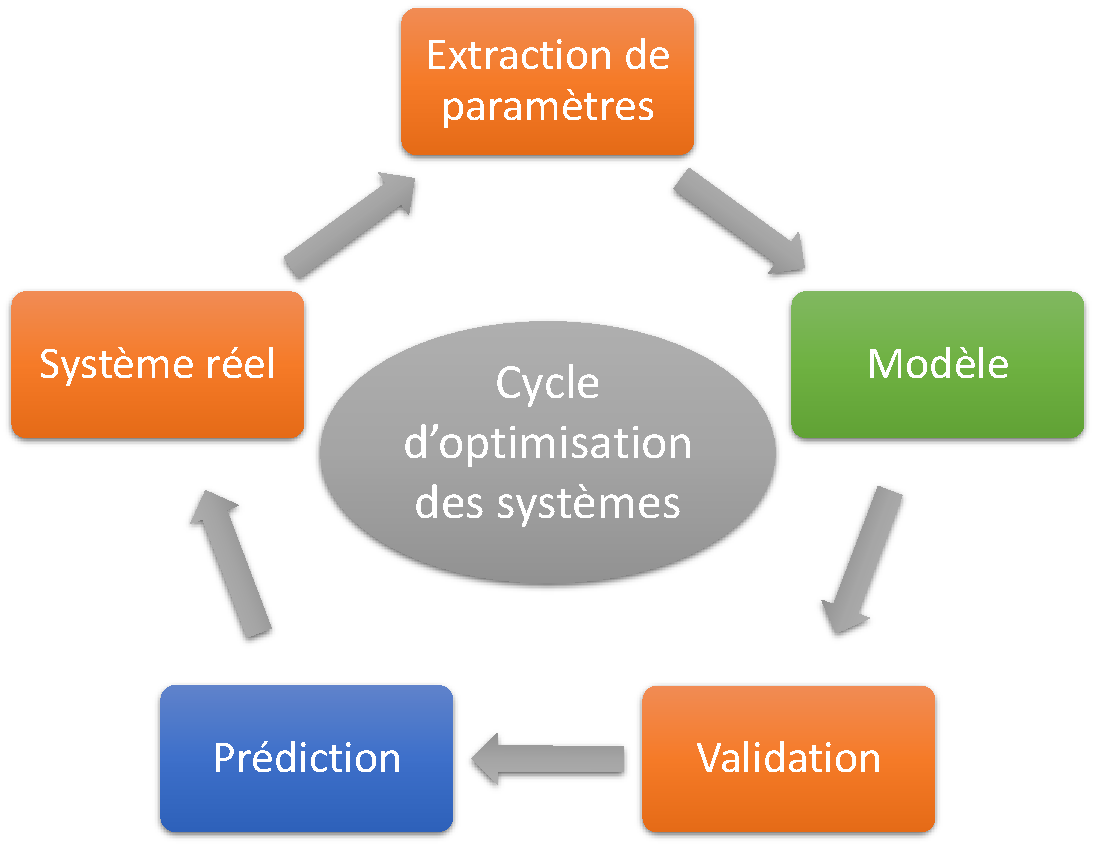
\includegraphics[scale=0.5]{chapitre3/chap3Fig/model-building.pdf}
 \caption{Le cycle d'optimisation éco-énergétique des systèmes informatiques.}
 \label{fig:model-building}
\end{figure}

La modélisation de l'énergie est un domaine de recherche actif. Il existe une panoplie des travaux dans la littérature, des revues comme \cite{Beloglazov11,Reda12,Ge13,Orgerie14,Dayarathna16} donne un aperçu global sur ces travaux sur plusieurs niveaux (architecture, système, composants, circuit, système d'exploitation, application, etc.) et avec une classification détaillée. Cependant, un modèle de coût énergétique de base peut être formuler comme suit :
\begin{equation}
 E = \alpha \; I_{cpu} + \beta \; I_{mem} + \gamma \; I_{es} + \delta \; I_{com} + \epsilon 
\end{equation} 
Où $I_{cpu}$, $I_{mem}$, $I_{es}$ et $I_{com}$ représentent le nombre d'instructions du processeur, l'utilisation de la mémoire, le débit d'E/S de disque et le nombre de transfert réseau respectivement. $\epsilon$ est une valeur d'erreur ou perturbation, qui représente les erreurs dans les mesures. Les poids $\alpha$, $\beta$, $\gamma$ et $\delta$ sont obtenus par une phase d'extraction de paramètres et l'étude du comportement des composants matériels sur la consommation d'énergie. Souvent, cette phase s'appuie sur les techniques d'apprentissage automatique \cite{Michalski13}.

% 4.2 Benchmarks: A Survey on Energy-Efficient Data Management
\subsubsection{Benchmarking}
Dans la deuxième catégorie des méthodes d’évaluation de l'énergie on trouve les benchmarks. Un indice de référence, ou benchmark, est un instrument d’analyse, de sensibilisation et de motivation des chercheurs. Il s’agit de définir des références pour se comparer aux meilleurs techniques de la branche d'EE, dans le but d’exploiter les potentiels d’amélioration en matière de gestion énergétique et de réaliser des économies \cite{Rivoire08phd}.

Les chercheurs, les agences gouvernementales et les consortiums standard de l'industrie pour les mesures de la performance, y compris \textit{Transaction Processing Performance Council} (\acrshort[hyper=false]{TPC}), \textit{Standard Performance Evaluation Corporation} (\acrshort[hyper=false]{SPEC}) et \textit{Storage Performance Council} (\acrshort[hyper=false]{SPC}) ont développé des benchmarks pour mesurer la consommation d'énergie des systèmes informatiques. Poess \textit{et al.} ont donné un aperçu très complet des benchmarks énergétiques actuellement disponibles. Il ont analysé leurs points communs et leurs différences selon diverses dimensions, y compris les composantes matérielles, la charge de requêtes et le type d'application, ainsi que les métriques et les exigences de précision et de calibration \cite{Poess10,PoessN08}.

\paragraph{TPC}
Le TPC a développé la norme \textit{TPC-Energy} \cite{Young10,TPCE} conçue pour augmenter les benchmarks de TPC existants avec des mesures d'énergie, afin que les utilisateurs finaux puissent comprendre les coûts d'énergie associés à un résultat d'un benchmark spécifique. Le nouvel benchmark répond à la demande émergente des mesures liées à l'énergie. Alors que TPC-C, TPC-E et TPC-CH ne fournissent que des mesures de performances, TPC-Energy introduit des mesures pour la consommation d'énergie pendant le traitement des requêtes. TPC-Energy régule en outre comment les mesures de puissance doivent être effectuées. Par exemple, quels sont les dispositifs de mesure à utiliser et quelle précision de mesure doit être maintenue. Les mesures définies par TPC-Energy sont la \textit{consommation d'énergie} par rapport au \textit{travail effectué} exprimée en \textit{Joule} par \textit{transaction} \cite{Schall11}.

\paragraph{SPEC}
SPEC a introduit le benchmark \textit{SPECpower\_ssj2008} \cite{SPECpowerssj2008} pour mesurer les performances et la consommation d'énergie d'un système exécutant des charges de travail basées sur Java. Le benchmark exerce les CPU, les caches, la hiérarchie de mémoire et l'évolutivité des processeurs de mémoire partagée sur plusieurs niveaux de charge. Le benchmark fonctionne sur une grande variété des systèmes d'exploitation et d'architectures matérielles avec la prise en charge des multi-nœuds. Contrairement à TPC-Energy, le benchmark SPEC mesure la consommation électrique de 0\% de charge à 100\% de charge et agrège les mesures par la moyenne géométrique pour former un seul résultat. En outre, les nouvelles versions du benchmark SPEC comme \textit{SPECweb\_2009} et \textit{SPECvirt\_sc2010} intègrent les méthodes de mesure de puissance de SPECpower.

\paragraph{SPC}
De plus, le SPC, dont les benchmarks sont focalisés sur l'évaluation des composants de stockage, a défini des extensions liées à l'énergie pour leurs benchmarks \cite{SPCBenchmark}. Ces extensions ne suivent pas la puissance maximale consommée à la charge, mais la mesurent à 80\% (notée intense) et 50\% (notée modérée) des performances maximales ainsi qu'en mode veille. En outre, ils introduisent la consommation d'énergie moyenne pondérée basée sur trois modes d'utilisation différents (faible, moyen et élevé).

\paragraph{Green500}
Le projet \textit{Green500} \cite{Green500} vise à la sensibilisation sur l'impact environnemental et à la durabilité à long terme des supercalculateurs haut de gamme en fournissant un classement des supercalculateurs les plus éco-énergétiques au monde. La liste de Green500 utilise << Performance par Watt >> comme métrique pour classer l'EE des supercalculateurs. La performance est définie comme la performance maximale obtenue, GFLOPS (Giga opération en virgule flottante par seconde), par le benchmark Linpack \footnote{\url{https://www.top500.org/project/linpack/}} sur l'ensemble du système. La puissance est définie comme la consommation d'énergie moyenne du système pendant l'exécution de Linpack.

\paragraph{JouleSort}
À part les benchmarks proposés par les organismes spécialisés, la communauté des bases de données elle-même a proposé un benchmark en matière d'énergie pour évaluer l'EE des systèmes informatiques. Le benchmark \textit{JouleSort} \cite{Rivoire07} est un benchmark de tri, dont l'idée est de mesurer l'énergie consommée pour trier une taille de données. Il mesure l'EE des systèmes à leur maximum d'utilisation (100\% de la charge). Il s'agit d'une extension du \textit{Sort Benchmark}\footnote{\url{http://sortbenchmark.org/}}, qui est utilisé pour mesurer la performance et le coût-performance des systèmes informatiques. JouleSort mesure le coût d'une certaine quantité de travail, avec une certaine mesure de consommation de puissance, par exemple : la puissance moyenne, la puissance de pic et l'énergie totale.

\subsection{Approches d'EE dans les systèmes informatiques}
Aujourd'hui, les enjeux de l'informatique éco-énergétique sont de plus en plus étudiés à tous les niveaux dans les infrastructures informatiques. Compte tenu d'une brève description des méthodes d'évaluation d'énergie dans les systèmes, nous présentons dans cette section un état de l'art des travaux d'EE des systèmes informatiques sur trois niveaux : (1) matériel, (2) système d'exploitation et (3) application. La \ref{fig:ee-it} illustre l'interdépendance des différents niveaux qui ont un impact sur la consommation d'énergie des systèmes informatiques.

\begin{figure}
 \centering
 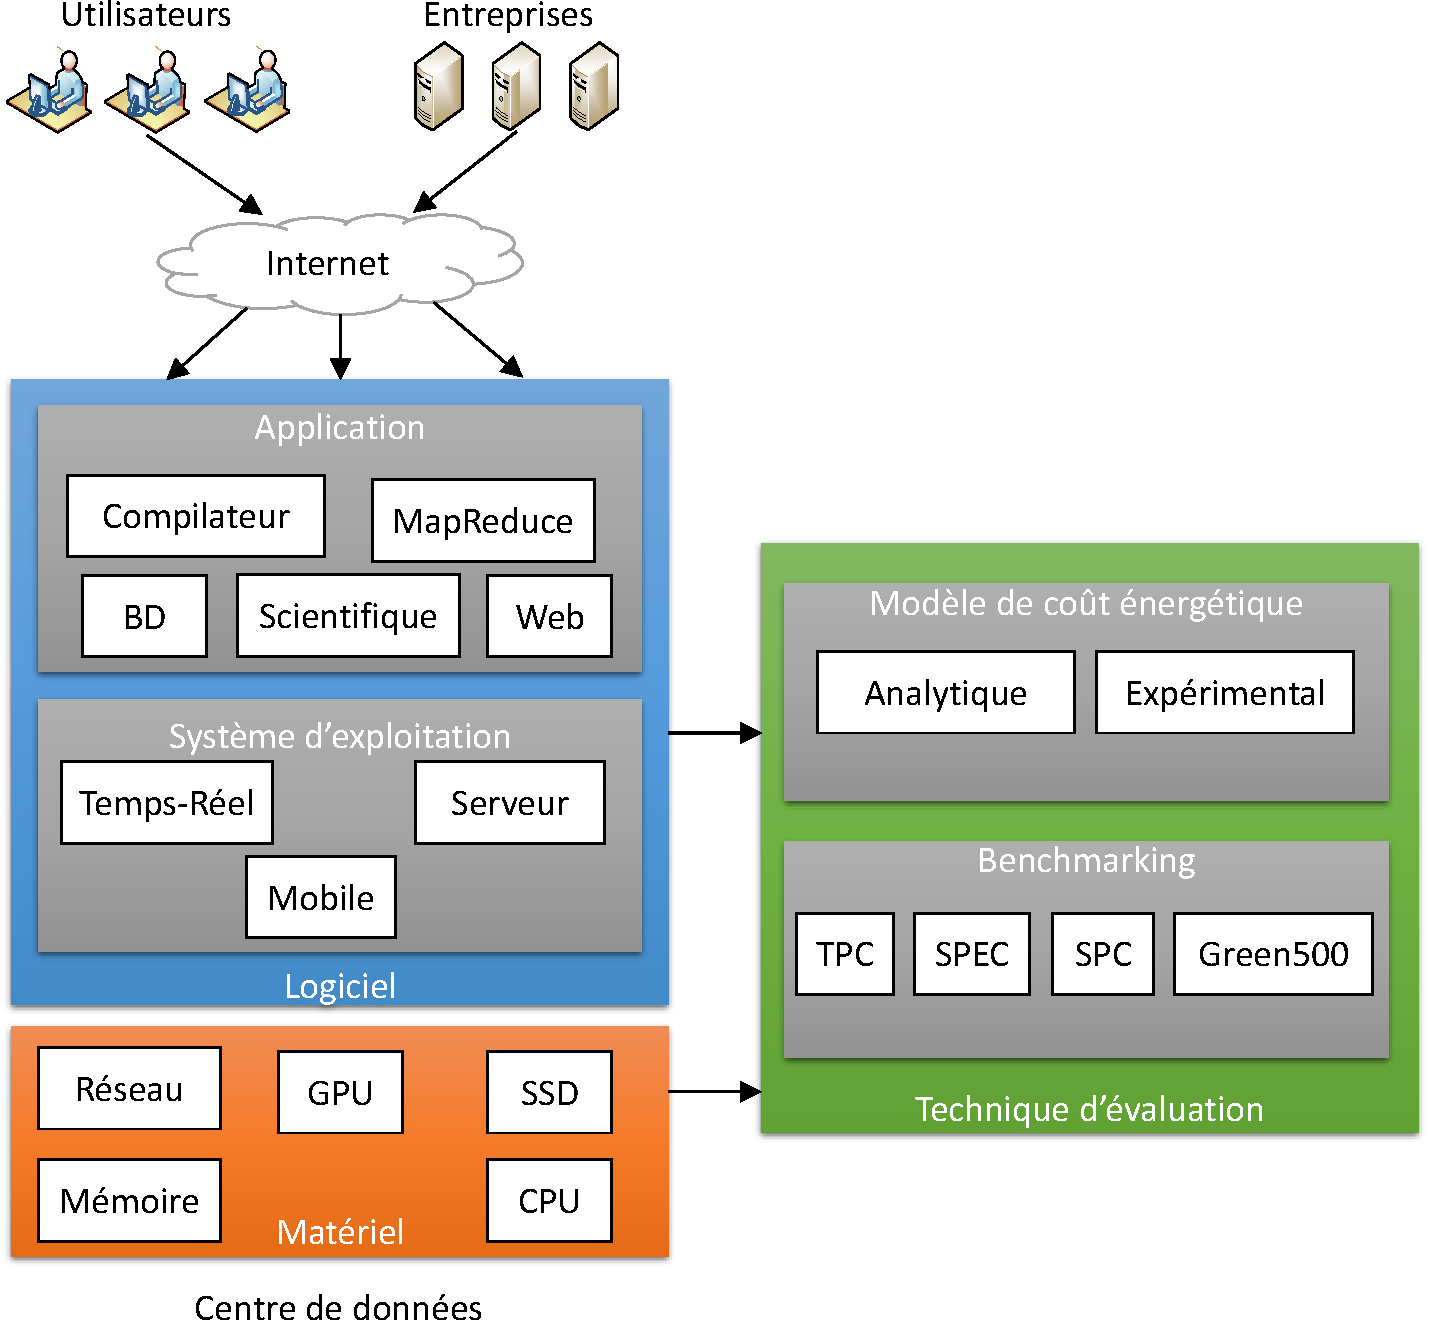
\includegraphics[scale=0.45]{chapitre3/chap3Fig/ee-it.pdf}
 \caption{La consommation d'énergie dans les systèmes informatiques sur les trois niveaux.}
 \label{fig:ee-it}
\end{figure}

\subsubsection{Approches d'EE au niveau matériel}
Un ordinateur de calcul comprend plusieurs composants, chacun pouvant être optimisé pour économiser l'énergie. Nous allons évoquer brièvement les techniques importantes proposées pour chaque composant.

Afin de réduire la consommation d'énergie du CPU, les auteurs de \cite{Weiser94} ont proposé un travail original. L'idée de base est le contrôle dynamique de la vitesse d'horloge pour réduire la consommation d'énergie pour un travail particulier. L'avantage provient de la réduction dans la tension électrique qui suit le ralentissement de l'horloge. Comme un inconvénient pour appliquer cette technique, le temps d'exécution augmente. Ce travail a largement inspiré le développement de la technique d'ajustement dynamique de la tension (DVS), et également la communauté des chercheurs. Encouragés par ces avantages, les chercheurs dans \cite{Yao95} ont construit un modèle théorique sur la base de travail précédent. L'objectif est de trouver le moyen le plus économe en énergie pour ordonnancer les tâches tout en respectant les délais d'exécution. L'ordonnancement heuristique en ligne des tâches apériodiques tout en conservant la faisabilité des ensembles de tâches périodiques est présenté dans \cite{Hong98}. Un algorithme éco-énergétique pour l'ordonnancement sans préemption est proposée dans \cite{Hong99}. Une autre méthode tente de ralentir le CPU à chaque fois qu'il y a une seule tâche éligible pour l'exécution, a été développée dans \cite{Shin99}. Une approche plus agressive est présentée dans \cite{Aydin01}, où deux algorithmes hors et en ligne sont considérés en respectant les délais, tout en réduisant la vitesse du cycle CPU autant que possible. Une comparaison systématique des différents algorithmes d'ordonnancement sur le rapport temps/performance est démontrée dans \cite{Govil95}. Dans \cite{Pillai01}, les informations de la date limite sont adoptées dans le système d'exploitation en temps réel avec la technique DVS. La norme ACPI  (\textit{Advanced Configuration and Power Interface}), disponible sur la plupart des systèmes d'exploitation, fournit une interface standard pour gérer les états de puissance du processeur \cite{Bergamaschi12}. Pour résumer, la plupart de ces algorithmes d'ordonnancement proposés tentent de tirer parti de l'EE et des contraintes temporelles d'un système en temps réel, à fin d'adapter le meilleur compromis raisonnable entre la tension électrique et les performances.

Par rapport à l'intérêt de la recherche dans l'utilisation du processeur, il y avait d'autres voix disant que le DVS peut-être également appliquée sur d'autres composantes, telle que la gestion de la mémoire. Les auteures de \cite{Fan03} illustrent par simulation que ni la gestion d'alimentation de mémoire ni encore la technique DVS sur le processeur, peuvent économiser l'énergie de façon spectaculaire. Mais en combinant les deux techniques ensemble, 89\% d'économie d'énergie, par rapport au cas de base, peut être achevé. Les techniques d'optimisation et les algorithmes proposés \cite{Lebeck00,Park11,Wu12} se sont concentrés sur les opportunités de basculer la mémoire entière ou une partie d'elle en mode faible consommation, soit pendant ou au moment de l'exécution des processus. D'autres technologies émergentes telles que la mémoire à changement de phase (PCM) \cite{Zhou09}, transfert de spin \cite{Wang08} et memristor \cite{Niu10} ont également été proposées comme des alternatives de la mémoire principale économe en énergie.

Les unités de traitement graphique (\acrshortpl[hyper=false]{GPU}) sont également devenues une partie essentielle des centres de données hébergeant des applications scientifiques à cause de leur efficacité dans les fonctions à virgule flottante. De plus, les GPUs sont très efficaces sur le plan énergétique par rapport aux processeurs. Les deux principales machines supercalculateur à haut rendement énergétique sont basées sur GPU \cite{Green500}. Les GPUs fournissent près de 85 fois moins de consommation d'énergie pour un calcul en virgule flottante que les processeurs x86 \cite{Keckler11}.

Il existe deux techniques de base pour atteindre l'EE dans les équipements de stockage : (1) rendre le matériel de stockage économes en énergie, et (2) réduire la redondance des données \cite{Yoder10}. Le principal objectif du matériel de stockage éco-énergétique est constitué par les disques SSDs (Solid-State Drive). Les disques SSD utilisent une mémoire Flash, c'est-à-dire une mémoire non volatile ayant des caractéristiques similaires à la mémoire morte effaçable électriquement et programmable (EEPROM). Les SSDs ont des propriétés proportionnelles à l'énergie, du fait que l'énergie utilisée est proportionnelle aux opérations d'E/S par seconde \cite{Shuja16}. D'autre part, les disques durs (HDDs) consomment 85\% d'énergie lorsqu'ils sont inactifs \cite{Narayanan09}. Les SSDs deviennent l'avenir du stockage primaire économe en énergie dans les systèmes.

Les périphériques réseau constituent une autre ressource énergétique dans les centres de données \cite{Orgerie14}. La consommation d'énergie dans les périphériques réseau peut être gérée par des techniques de taux de liaison adaptatif (ALR) \cite{Bilal13,Bilal14}. Les techniques d'ALR atteignent l'EE par : (1) des débits de données réduits, ou (2) des transitions d'état de puissance inférieure/inactive qui sont gérées en fonction des charges de données \cite{Bilal13b}. Les protocoles de routage efficaces jouent un rôle important dans l'utilisation de la capacité réseau. Shang \textit{et al.} \cite{Shang10} ont avancé l'idée du routage énergétique où peu de périphériques réseau fournissent le routage de base et le débit en fonction d'un seuil de performance tandis que le reste des périphériques sont hors tension.

\subsubsection{Approches d'EE au niveau système d'exploitation}
La communauté de la recherche a rapidement réalisé l'impact significatif de la couche système sur la consommation d'énergie. Le travail de \cite{Benini00} classe les composants du système consommant la majeure partie de l'énergie en trois catégories : unités de calcul, unités de communication et unités de stockage. Les auteurs présentent également un état de l'art des techniques éco-énergétique autour de trois phases principales d'une conception de système : la conceptualisation et la modélisation, la conception et la mise en œuvre, et la gestion d'exécution. Les recherches montrent ainsi que les systèmes d'exploitation (SE) ont une consommation d'énergie hétérogène et peuvent-être optimisés pour consommer moins d'énergie. La consommation varie même entre les versions du même SE. Par exemple, la consommation d'un ordinateur sous différentes versions de Windows et des noyaux Linux, suivent des méthodologies de mesures similaires, présente des variations non négligeables \cite{Orgerie14}. Les auteurs de \cite{Pallipadi06} ont développé un gestionnaire d'alimentation en temps réel dans le noyau pour le système d'exploitation Linux appelé le gouverneur à la demande (LGD). Le gestionnaire surveille en permanence l'utilisation du processeur et définit une fréquence d'horloge qui correspond aux exigences de performances actuelles, ce qui minimise la consommation d'énergie. Le travail de \cite{Zeng02} a proposé et développé \textit{ECOsystem}, un framework pour la gestion de l'énergie en tant que ressource de première classe dans un SE destinée aux dispositifs alimentés à l'aide de batterie tels que les mobiles. ECOsystem fournit une interface pour définir une durée de vie de la batterie cible et des priorités d'application utilisées pour déterminer la quantité d'énergie qui sera allouée aux applications à chaque période. Des techniques similaires ont été proposées pour les mobiles comme : \textit{Nemesis OS} \cite{Neugebauer01}, \textit{GRACE} \cite{Sachs04,Vardhan09} et \textit{Coda/Odyssey} \cite{Flinn04}, et pour les serveurs : \textit{Linux/RK} \cite{Rajkumar97}, \textit{PowerNap} \cite{Meisner09} et \textit{Barely Alive} \cite{Anagnostopoulou12}.

\subsubsection{Approches d'EE au niveau application}
L'EE au niveau application est devenu un domaine de recherche actif pour les raisons suivantes : (1) les techniques d'optimisation de bas niveau (matériel et SE) dépend fortement de l'estimation précise des profils de puissance des applications. Cependant, beaucoup d'informations et de statistiques nécessaires pour ces estimations ne sont disponibles que dans le niveau application. (2) De nombreuses applications peuvent être exécutées de différentes manières pour accomplir la même tâche de calcul. Les applications éco-énergétique, qui adaptent leurs comportements en fonction des états liés à l'alimentation des systèmes sous-jacents, peuvent offrir des possibilités supplémentaires d'économie d'énergie. De nombreux projets de recherche dans ce domaine sont consacrés aux services Web \cite{Bohrer02,Sharma03,Chase01,Chen05}, les compilateurs \cite{Hsu03,Huang07,Kadayif05} et les environnements de développement (EDI) \cite{Capra12}. Dans \cite{Xian07}, un framework de programmation à usage général a été développé pour permettre aux applications d'être exécutées avec des plans différents en fonction de leurs coûts d'énergie. \textit{SEEDS} est un framework pour aider les ingénieurs des logiciels à développer des applications éco-énergétiques de haut niveau \cite{Manotas14}. SEEDS fournit une analyse automatisée, une prise de décision et une mise en œuvre visant à optimiser la consommation d'énergie d'une application donnée. Une application récente des techniques éco-énergétique inclut \textit{MapReduce} \cite{Chen12,Lang10,Leverich10}.

Et encore plus récemment, la consommation d'énergie dans les bases de données commence à attirer l'attention de la communauté des chercheurs. L'objectif principal de ces efforts est de concevoir des SGBDs avec la consommation optimisée d'énergie. Notre étude s'inscrit dans cette catégorie, et nous allons détailler dans une section séparée les différents travaux de littérature sur l'EE dans les bases de données. La \ref{fig:energy-approaches-classification} représente une classification des travaux d'EE dans les systèmes informatiques sur les trois niveaux discutés.

\begin{figure}
\footnotesize
\begin{center}
\tikzset{
  basic/.style  = {draw, text width=4cm, drop shadow, rectangle},
  root/.style   = {basic, rounded corners=2pt, thin, align=center,
                   fill=green!30},
  level 2/.style = {basic, rounded corners=6pt, thin,align=center, fill=green!60,
                   text width=8em},
  level 3/.style = {basic, thin, align=left, fill=pink!60, text width=8.5em}
}
\begin{tikzpicture}[
  level 1/.style={sibling distance=50mm},
  edge from parent/.style={->,draw},
  >=latex]

% root of the the initial tree, level 1
\node[root] {Approches d'EE dans les systèmes informatiques}
% The first level, as children of the initial tree
  child {node[level 2] (c1) {Niveau matériels}}
  child {node[level 2] (c2) {Niveau SE}}
  child {node[level 2] (c3) {Niveau application}};

% The second level, relatively positioned nodes
\begin{scope}[every node/.style={level 3}]
\node [below of = c1, xshift=15pt] (c11) {CPU \cite{Weiser94,Yao95,Hong98,Hong99,Shin99,Aydin01,Pillai01,Bergamaschi12}};
\node [below of = c11] (c12) {Mémoire \cite{Fan03,Lebeck00,Park11,Wu12,Zhou09,Wang08,Niu10}};
\node [below of = c12] (c13) {GPU \cite{Keckler11,Green500}};
\node [below of = c13] (c14) {Stockage \cite{Yoder10,Shuja16,Narayanan09}};
\node [below of = c14] (c15) {Réseau \cite{Orgerie14,Bilal13,Bilal14,Bilal13b,Shang10}};

\node [below of = c2, xshift=15pt] (c21) {LGD \cite{Pallipadi06}};
\node [below of = c21] (c22) {Mobiles \cite{Zeng02,Neugebauer01,Sachs04,Vardhan09,Flinn04}};
\node [below of = c22] (c23) {Serveurs \cite{Rajkumar97,Meisner09,Anagnostopoulou12}};

\node [below of = c3, xshift=15pt] (c31) {Services Web \cite{Bohrer02,Sharma03,Chase01,Chen05}};
\node [below of = c31] (c32) {Compilateurs \cite{Hsu03,Huang07,Kadayif05}};
\node [below of = c32] (c33) {EDI \cite{Capra12,Manotas14}};
\node [below of = c33] (c34) {MapReduce \cite{Chen12,Lang10,Leverich10}};
\node [below of = c34] (c35) {Base de données};
\end{scope}

% lines from each level 1 node to every one of its "children"
\foreach \value in {1,...,5}
  \draw[->] (c1.178) |- (c1\value.west);

\foreach \value in {1,...,3}
  \draw[->] (c2.178) |- (c2\value.west);
  
\foreach \value in {1,...,5}
  \draw[->] (c3.178) |- (c3\value.west);
\end{tikzpicture}
\caption{Classification des approches d’EE dans les systèmes informatiques.}
\label{fig:energy-approaches-classification}
\end{center}
\end{figure}

\section{Approches d'EE dans les BD}
%La gestion de l'énergie des systèmes de bases de données est devenue un sujet de recherche important au cours des dernières années. Les travaux de recherche proposés comprennent à la fois les dimensions matérielles et logicielles.
%Deux hypothèses principales ont été retenues pour ces initiatives: (i) applications de base de données déjà déployées ($\mathcal{BDDD}$) et (ii) applications de base de données non déployées ($\mathcal{BDND}$). Dans la première hypothèse, nous considérons que l'application de base de données est déjà conçue et déployée sur une plate-forme donnée. En ce qui concerne les initiatives avec l'hypothèse de $\mathcal{BDND}$, la majorité des études couvrent la partie matériel. Dans cet thèse, nous nous concentrons uniquement sur une initiative concernant les techniques logicielles avec l'hypothèse $\mathcal{BDDD}$.

La gestion de l'énergie des systèmes de bases de données est devenue un sujet de recherche important au cours des dernières années. Il y a eu une pléthore d'études et d'initiatives de la communauté des chercheurs. Lors de l'étude de la littérature des travaux, on distingue principalement deux approches principales : \textit{Approches Orientées Matériels} ($\mathcal{\acrshort[hyper=false]{AOM}}$) et \textit{Approches Orientées Logicielles} ($\mathcal{\acrshort[hyper=false]{AOL}}$). Dans les sections suivantes, nous détaillons les travaux de chaque approche.
%comme le montre la Figure . %Dans cette section, nous proposons une enquête et une classification de ces approches, comme le montre la \ref{fig:energy-approaches-classification}.

\subsection{$\mathcal{AOM}$}
Les approches matérielles utilisent des solutions << naïves >> comme la désactivation de composants électroniques pendant les périodes d'inactivité, et des solutions avancées telles que la modification dynamique de la performance des composants matériels pour une meilleure EE, qui peut être illustrer par la technique DVFS offerte par les CPU d'aujourd'hui \cite{Beloglazov11}. Par ailleurs, les techniques appliquées au niveau du matériel peuvent être divisées en deux catégories: (i) dispositif de traitement et (ii) la gestion du stockage.

\subsubsection{Dispositif de traitement}
Les techniques appartenant à cette catégorie utilisent de nouvelles approches pour minimiser la consommation d'énergie des appareils informatiques.
Lang \textit{et al.} ont proposé le mécanisme PVC (Processor Voltage/Frequency Control) pour équilibrer la consommation d'énergie et la performance \cite{Lang09}. Il vise à exécuter des instructions à une tension et une fréquence de processeur basse en tirant parti de la capacité des processeurs modernes. Une technique similaire est utilisée dans \cite{Tu14}, les auteurs rapportent 51,3\% des économies d'énergie. La technique proposée ajuste dynamiquement le niveau DVFS du processeur en fonction des performances du SGBD ou le plan de requête choisi pour l'exécution. Xu \textit{et al.} \cite{Xu13b} aussi utilisent la technique DVFS avec un mécanisme de contrôle de rétroaction pour les charges de requêtes d'une base de données. Afin d'économiser l'énergie, ils gèrent le niveau DVFS en fonction du débit de travail (\textit{throughput}) et des caractéristiques de la charge de requêtes (par exemple, en basant sur le nombre d'E/S ou de CPU). Dans une autre étude, une co-ingénierie entre Oracle et Intel tente de réduire les coûts d'exploitation et de répondre efficacement aux objectifs d'informatique durable (\textit{green computing}) a donné lieu à une nouvelle version de \textit{Oracle Exadata Database Machine} \cite{IntelOracle14}. La solution proposée met dynamiquement le processeur Intel Xeon et la mémoire dans l'état de puissance disponible le plus bas convenable pour répondre aux exigences de la charge de requêtes. Cependant, les techniques mentionnées ci-dessus souffrent des frais additionnels pour la transition vers des états de faible puissance, qui conduisent généralement à une consommation d'énergie supplémentaire et des délais d'exécution causés par la réinitialisation des composants \cite{Beloglazov11}.

Pour accélérer les applications de données intensives, les Field-Programmable Gate Array (FPGA) sont utilisés à la place des processeurs classiques, principalement parce qu'ils permettent la construction de matériel personnalisé à des coûts de développement relativement faibles. De plus, il a déjà été montré dans \cite{Woods14} que les solutions à base de FPGA ont le potentiel d'améliorer la performance et en même temps de réduire la consommation d'énergie. Les auteurs rapportent que l'utilisation de ces propositions pour certaines requêtes, permet au système de consommer que 216 \textit{Joules}, alors que les techniques traditionnelles consomment 3888 \textit{Joules}.

Les unités de traitement graphique (GPU) ont été considérées comme une excellente alternative aux processeurs pour leur haute performance, leur haut débit de traitement ainsi que leur économie d'énergie. Une étude a rapporté que l'utilisation d'un GPU est plus économe en énergie lorsque l'amélioration de la performance est supérieure à une certaine borne, par rapport à une solution CPU classique \cite{Rofouei08}. Le CPU-GPU co-traitement est une autre tendance intéressante dans la technologie de base de données, qui consiste à exploiter les avancées matérielles ainsi que la conception d'algorithmes optimisés pour améliorer les performances de traitement des requêtes et l'EE. Les résultats de comparaison entre une architecture CPU-GPU discrète et une architecture CPU-GPU couplée montrent que la consommation moyenne d'énergie de l'architecture discrète est entre 36\% et 44\% supérieurs à celle de l'architecture couplée \cite{Hurson16}.

D'autre part, des études récentes telles que \cite{Do13} affirment que l'utilisation de disques Smart Solid State (SSSDs) pour traiter les données peuvent-être plus avantageux à la fois en terme de performance et de consommation d'énergie. Les SSSDs se sont des dispositifs de stockage flash qui intègrent une mémoire et un processeur à l'intérieur du dispositif de SSD, et pourrait être utilisé pour exécuter des programmes généraux définis par l'utilisateur. Les auteurs de \cite{Do13} améliorent l'EE du traitement des requêtes en réduisant son temps d'exécution et/ou en exécutant le traitement sur le processeur de faible puissance qui vient avec les SSSDs. Les premiers résultats de l'exécution d'un sous-ensemble de requêtes SQL (simples requêtes de sélection et d'agrégation) sur un SSSD fournissent jusqu'à 3x de réduction de la consommation d'énergie. Les SSSD ont beaucoup de potentiel, mais les capacités de calcul des appareils embarqués dans les SSSD actuels sont trop limitées pour gérer le volume de données énormes.

\subsubsection{Gestion du stockage}
Les dispositifs de traitement ont été considérés comme les principaux contributeurs à la consommation d'énergie dans un serveur. Cela dit, la consommation d'énergie des dispositifs de stockage secondaire et de la mémoire ont également attiré une forte attention des chercheurs en raison de leurs capacités de croissance significative au cours des dernières années.
Les approches de gestion de stockage tentent de trouver un bon niveau de consolidation de la charge, l'amélioration des techniques de mise en cache et de préchargement et l'optimisation des modes d'alimentation dans les matrices de disques afin de minimiser la dissipation d'énergie \cite{Tu14}. Dans \cite{Harizopoulos09}, les auteurs fournissent des expériences pour montrer que les choix effectués par les systèmes de base de données peuvent améliorer l'EE. Plus précisément, repartitionner la base de données sur 66 disques propose une augmentation de 14\% de l'efficacité contre la dégradation de 45\% de la performance. Les auteurs de \cite{Tu14} ont proposé un modèle d'optimisation intégrée pour la migration des données et l'ajustement de l'état du disque, dans lequel ils placent dynamiquement les enregistrements dans un fragment selon la fréquence des enregistrements de données d'accès. Les résultats présentés montrent que près de 50\% de l'énergie peut être économisé en utilisant les techniques proposées. Dans la même direction, le travail de \cite{Behzadnia16} propose un modèle de gestion de puissance dynamique qui prend des décisions en temps réel sur le passage des disques à des modes de faible puissance. Le modèle est intégré dans le SGBD et utilisé pour obtenir le compromis optimal entre la consommation d'énergie et le temps de réponse des requêtes. Le rapport montre 60\% des économies d'énergie.

L'utilisation de disques SSD comme un périphérique de stockage des bases de données pour améliorer l'EE est une autre direction qui a été étudiée par des travaux récents. Dans \cite{Schall10}, les auteurs ont étudié le comportement de la performance et la consommation d'énergie des SSD pour des schémas d'accès typiques pour les applications de base de données à forte intensité d'E/S. Ils montrent, en outre, que la technologie SSD offre un nouveau niveau de performance et d'EE, et suggèrent l'exploitation de leurs nouvelles caractéristiques par les serveurs de base de données. De même, le travail de \cite {Cheong12} analyse et évalue les performances de traitement des données et l'EE des SSD et système de stockage. Comme son prédécesseur, les auteurs montrent l'amélioration de la performance et l'EE.

\begin{figure}
\footnotesize
\begin{center}
\tikzset{
  basic/.style  = {draw, text width=4cm, drop shadow, rectangle},
  root/.style   = {basic, rounded corners=2pt, thin, align=center,
                   fill=green!30},
  level 2/.style = {basic, rounded corners=6pt, thin,align=center, fill=green!60,
                   text width=8em},
  level 3/.style = {basic, thin, align=left, fill=pink!60, text width=8.5em}
}
\begin{tikzpicture}[
  level 1/.style={sibling distance=50mm},
  edge from parent/.style={->,draw},
  >=latex]

% root of the the initial tree, level 1
\node[root] {Approches orientées matériels}
% The first level, as children of the initial tree
  child {node[level 2] (c1) {Dispositif de traitement}}
  child {node[level 2] (c2) {Gestion du stockage}};

% The second level, relatively positioned nodes
\begin{scope}[every node/.style={level 3}]
\node [below of = c1, xshift=15pt] (c11) {CPU \cite{Lang09,Tu14,Xu13b,IntelOracle14,Beloglazov11}};
\node [below of = c11] (c12) {GPU \cite{Rofouei08}};
\node [below of = c12] (c13) {FPGA \cite{Woods14}};
\node [below of = c13] (c14) {Co-Traitement \cite{Hurson16,Do13}};

\node [below of = c2, xshift=15pt] (c21) {HDD \cite{Tu14,Harizopoulos09,Behzadnia16}};
\node [below of = c21] (c22) {SSD \cite{Schall10,Cheong12}};
\node [below of = c22] (c23) {Mémoire \cite{Appuswamy15,Korkmaz15,Xu10b}};
\end{scope}

% lines from each level 1 node to every one of its "children"
\foreach \value in {1,...,4}
  \draw[->] (c1.178) |- (c1\value.west);

\foreach \value in {1,...,3}
  \draw[->] (c2.178) |- (c2\value.west);
\end{tikzpicture}
\caption{Classification des approches d’EE orientées matériels.}
\label{fig:hardware-approaches-classification}
\end{center}
\end{figure}

La mémoire est un autre consommateur d'énergie important dans les systèmes informatiques, en particulier avec l'utilisation croissante des bases de données orientée colonnes où le stockage des données se fait directement dans la mémoire. De nombreux travaux de recherche récents commencent à étudier l'impact du dispositif de mémoire sur la consommation d'énergie. L'enquête faite dans \cite{Appuswamy15} souligne que l'utilisation croissante des bases de données en mémoire va bientôt émerger la mémoire en tant que consommateur de puissance électrique dominante au lieu de CPU. Comme pour les composants précédents, la mémoire principale a également des différents états de puissance et de la fréquence à modifier en fonction de son utilisation. Sur cette base, les auteurs ont utilisé la fréquence mise à l'échelle et des modes de mise hors tension des DRAM pour améliorer la consommation d'énergie sans sacrifier les performances. Dans \cite{Korkmaz15}, les auteurs rapportent un résultat préliminaire sur une technique d'allocation de mémoire basée sur les rangs pour économiser l'énergie des systèmes de base de données. La technique permet au SGBD de déplacer les rangs inutiles de la mémoire aux états de faible puissance et réduire ainsi la consommation d'énergie globale. L'évaluation indique que la méthode proposée atteint 40\% de diminution de la puissance lorsque la taille de la base de données est plus petite que la quantité de la mémoire déjà provisionnée sur le serveur. Le travail de \cite{Hassan15} propose une architecture de mémoire hybride comprenant à la fois Dynamic Random Access Memory (DRAM) et de la mémoire non volatile (NVM) pour réduire la consommation d'énergie de base de données, grâce à une politique de gestion des données au niveau de l'application qui décide de placer des données sur la DRAM ou la NVM. Ils analysent d'abord l'exécution d'applications et de collectent des statistiques d'accès mémoire pour des objets individuels. Ceux-ci sont évalués en utilisant un modèle d'analyse de la performance et de l'énergie pour identifier la technologie de mémoire la plus adaptée pour stocker ces données. Les résultats présentés indiquent que l'utilisation de la mémoire hybride peut réduire l'énergie du système de mémoire d'environ 80\%.

\subsection{Bilan et discussion}\label{sec:bilanAOM}
Dans les sections précédentes, nous avons classé les techniques appliquées au niveau du matériel en deux catégories, dispositif de traitement et la gestion du stockage. Les études précitées dans pour chaque catégorie ont en effet apporté une contribution importante à la conservation de l'énergie (voir \ref{fig:hardware-approaches-classification}). Cependant, les $\mathcal{AOM}$ ne sont pas simple à appliquer et ont plusieurs inconvénients en particulier dans le domaine des bases de données. Tout d'abord, ils ont besoin d'utiliser du nouveau matériel, puisque les nouvelles technologies tels que DVFS ne sont pas disponibles sur tous les processeurs ou mémoires actuels. Deuxièmement, les SSD émergents sont très chers et ont un problème de durée de vie. Dernier point, mais non des moindres, il existe différentes marques/versions pour chaque composant matériel, ce qui rend ces méthodes peu pratiques en raison de leurs problèmes de portabilité.
Par conséquent, les $\mathcal{AOL}$ sont beaucoup préférés dans le cadre des bases de données, car ils sont indépendants du matériel sous-jacent. En outre, le SGBD a une connaissance détaillée des éléments internes du système, tels que la charge de requêtes, les plans d'exécution, les statistiques de base de données, etc. \cite{Korkmaz15}. Dans \cite{Harizopoulos09}, Harizopoulos \textit{et al.} de laboratoire de HP confirment que << les approches matérielles ne sont qu'une partie de la solution, et les approches logicielles seront la clé dans l'optimisation de l'efficacité énergétique >>.

\subsection{$\mathcal{AOL}$}
Les approches matérielles ne sont qu'une partie de la solution pour réduire les valeurs de puissance; les approches logicielles sont l'autre élément clé dans les mécanismes d'optimisation de l'EE. A ce niveau, les papiers de vision sur l'énergie \cite{Graefe08, Harizopoulos09} recommandent de revoir les techniques d'optimisation des requêtes, les algorithmes d’ordonnancement, la conception physique et les techniques de mise à jour de base de données en tenant compte de l'énergie. La plupart des importantes études concernent deux aspects principaux : (i) la définition des modèles de coûts pour prédire l'énergie et (ii) la proposition des techniques basées sur les modèles de coûts pour réduire l'énergie. Cette situation est tout à fait semblable à celle vécue dans les approches de conception traditionnelles axées sur l'amélioration de la performance, où la plupart des optimiseurs de requêtes des SGBD open source \footnote{\url{http://www.postgresql.org/docs/current/static/planner-optimizer.html}} et commerciale \footnote{\url{http://docs.oracle.com/cd/B10500_01/server.920/a96533/optimops.htm\#51003}} utilisent des approches fondées sur les modèles de coûts. Dans ces approches, un optimiseur basé sur les coûts estime le coût de chaque plan d'exécution possible en appliquant des formules heuristiques utilisant un ensemble de statistiques relatives à la base de données (taille des tables, des indexes, longueur de tuples, les facteurs de sélectivité de jointure et prédicats de sélection, la taille des résultats intermédiaires, etc.) et au matériel (taille du tampon mémoire, la taille de page, etc.).

\subsubsection{Définition des modèles de coûts}
Dans \cite{Xu13, Xu10b}, les auteurs proposent une extension du modèle de coût de PostgreSQL pour prédire la consommation d'énergie d'une seule requête exécutée d'une façon isolée (pas de parallélisme inter-requêtes). Un profil de puissance statique pour chaque opération de base de données basique est défini dans la phase du traitement des requêtes. Le coût de l'énergie d'un plan peut être calculé à partir des opérations de base de données SQL, comme le coût de la puissance du processeur pour accéder à un tuple, coût du disque pour la lecture/écriture d'une page et ainsi de suite, et par l'intermédiaire de différentes méthodes d'accès et d'opérations de jointure, en utilisant une technique de régression linéaire simple. La formule générale pour calculer l'énergie d'un opérateur $x$ est :
\begin{equation}
\hat{E}_x = W_{cpu} \times N_{tuples}^{m} \times N_{tuples} + \bar{W}_{E/S} \times N_{pages}
\end{equation}
Où $W_{cpu}$ et $\bar{W}_{E/S}$ sont le coefficient de consommation d'énergie d'un tuple traité par le CPU ($N_{tuples}$), et le coefficient statique d'une page traitée en E/S ($N_{pages}$), et $m$ est un coefficient de modèle pour la consommation d'énergie du CPU ($m = 0,5$ après la régression).
Les auteurs adaptent leur modèle statique pour des charges de requêtes dynamiques à l'aide d'un mécanisme de contrôle de rétroaction pour mettre à jour périodiquement les paramètres du modèle à travers des mesures d'énergie en temps réel.

Dans \cite{Kunjir12}, une recherche profonde dans la modélisation de la puissance de pic des opérations de requête est donnée. Un modèle de plans d'exécution sur la base de pipeline a été développé pour identifier les sources de consommation d'énergie de pic pour une requête isolée et de recommander des plans avec une faible puissance de pic. Pour chacun de ces pipelines, une fonction mathématique est appliquée, qui prend en entrée les taux et les tailles des données circulant à travers les opérations de pipelines. En tant que sortie, une estimation de la consommation d'énergie de pic est donné. Les auteurs ont utilisé la technique de régression multiple affine par morceaux pour construire leurs modèles de coût. Pour un nœud de base $B$ (par exemple : un accès séquentiel), le débit est calculé comme :
\begin{equation}
 Taux_B = \frac{Entrée_B}{TempsDisque_B}
\end{equation}
Où $Entrée_B$ indique la taille des données extraites du disque par $B$ et $TempsDisque$ est le temps de transfert du disque.
\begin{alignat}{2}
& \text{soit}  \quad && Base_N = SousArbre^{PL}_{N} \cap Base^{PL} \nonumber \\
& \text{alors} \quad && Taux_N = \frac{\sum_{i \in Source^{PL}_{N}} Sortie_i}{max_{x \in Base_N} TempsDisque_x}
\end{alignat}
$N$ est un nœud générique en aval dans le pipeline, $SousArbre^{PL}_{N}$ est le sous-arbre du pipeline $PL$ avec la rince $N$, $Base^{PL}$ est l'ensemble des nœuds de bases dans le pipeline $PL$, $Source^{PL}_{N}$ est l'ensemble des nœuds dans le pipeline $PL$ qui fournissent directement des entrées au nœud $N$, et $Sortie_i$ désigne la taille de la donnée en sortie par le nœud $i$. Les tailles des données sont estimées à partir de catalogue de la base de données.

Dans le même sens, le travail de \cite{Lang11} propose un framework pour un traitement éco-énergétique des requêtes dans les bases de données. Il étend les plans de requêtes produites par l'optimiseur de requête traditionnelle avec une prédiction de la consommation d'énergie pour certains opérateurs de bases de données spécifiques comme la sélection, projection et la jointure en utilisant la technique de régression linéaire. L'\ref{eq:lang11} montre le modèle le plus précis proposé pour estimer la puissance moyenne du système pendant l'exécution d'une requête isolée. Le modèle est défini par trois types de variables :
\begin{enumerate}
 \item Temps $T$
 \item Paramètres de requête $Q$ : nombre d'instructions de processeur ($I_Q$), lecture de page disque ($R_Q$), écriture de page disque ($W_Q$) et nombre d'accès au mémoire ($M_Q$)
 \item Paramètres du système : CPU ($C_{cpu}$), lecture disque ($C_R$), écriture disque ($C_W$), accès mémoire ($C_{mm}$), reste du système ($C_{autres}$). Ces paramètres quantifient la puissance des composants matériels et sont obtenus par une régression.
\end{enumerate}

\begin{equation}\label{eq:lang11}
 P_{moy} = C_{cpu} \times \frac{I_Q}{T} + C_R \times \frac{R_Q}{T} + C_W \times \frac{W_Q}{T} + C_{mm} \times \frac{M_Q}{T} + C_{autres}
\end{equation}

L'intuition derrière ce modèle est de calculer la sommation de la puissance moyenne du processeur ($C_{cpu} \times \frac{I_Q}{T}$), du lecture disque ($C_R \times \frac{R_Q}{T}$), d'écriture disque ($C_W \times \frac{W_Q}{T}$), du mémoire ($C_{mm} \times \frac{M_Q}{T}$) et du reste du système ($C_{autres}$) pendant l'exécution de la requête $Q$.

L'étude de \cite{Rodriguez11} tente de modéliser l'énergie et la puissance de pic des requêtes de sélection simples sur les relations individuelles en utilisant une régression linéaire. Le modèle développé pour la consommation d'énergie d'une requête $Q$ avec une relation $R$ est le suivant :
\begin{equation}
 E_Q = \beta_0 + \beta_1 \; S + \beta_2 \; SF_p(R) \; S + \beta_3 \; |R| \; SF_p(R) + \beta_4 \; |R| <R> SF_p(R)
\end{equation}

Où $\beta_i$ sont des coefficients de régression et $|R|$, $<R>$, $SF_p(R)$ et $S$ sont respectivement : la cardinalité de la relation $R$, le nombre de colonnes de $R$, la sélectivité du prédicat $p$ dans $R$ et le nombre de serveurs utilisés. Les requêtes sont supposées exécuter d'une façon isolée.

Alors que les travaux cités considèrent seulement une architecture de base de données centralisée, l'étude de Lang \textit{et al.} \cite{Lang12} a proposé un modèle de coût pour une architecture de base de données en grappe de serveurs. Le modèle prend en compte les configurations de serveur (par exemple, le CPU, les disques et la bande passante du réseau) et les paramètres de traitement de données (par exemple, la sélectivité des prédicats, la taille de la table de hachage), et prédit les performances de traitement des données et l'EE pour un opérateur de jointure par hachage. L'erreur maximale rapportée est inférieure à 10\%.

\subsubsection{Techniques basées sur des modèles de coûts}
Les modèles de coûts proposés pour prédire l'énergie sont ensuite utilisés dans diverses techniques pour optimiser la consommation d'énergie de base de données. Les auteurs de \cite{Lang09} ont proposé un mécanisme pour améliorer l'EE des requêtes en introduisant des retards explicites, en utilisant l'agrégation des requêtes pour tirer parti des composants de requêtes communs dans la charge. Le retard explicite permet de grouper les requêtes dans une file d'attente en mémoire tampon, ce qui conduit alors à une évaluation plus efficace de l'ensemble du lot par des techniques d'optimisation multi-requêtes. Pour la comparaison de l'énergie et du temps, la métrique utilisée est le Produit Énergétique/Délai (\acrshort[hyper=false]{EDP}) \cite{Laros13}, qui est le produit de l'énergie et du délai : 
\begin{equation}\label{eq:edp}
 EDP = \text{énergie} (Joules) \times \text{temps} (sec)
\end{equation}
Après la substitution, la formule finale de comparaison est :
\begin{equation}
 EDP = V^2 / F
\end{equation}
Où $V$ est le voltage et $F$ est la fréquence du processeur. Les résultats d'expérimentations pour les requêtes de sélection simples montrent que cette technique peut être utilisé pour trouver un compromis entre la performance et l'énergie, ce qui réduit la consommation d'énergie de 54\% contre 43\% d'augmentation dans le temps de réponse moyen.

Le travail de \cite{Psaroudakis14} indique que l'ordonnancement éco-énergétique de plusieurs requêtes peut améliorer l'EE de certains opérateurs SQL basique qui peuvent être exécutées en parallèles, tels que les agrégations et les algorithmes d'accès aux données. La métrique utilisée pour choisir le meilleur compromis entre le temps et l'énergie est EDP (\ref{eq:edp}). Les résultats expérimentaux montrent que l'application des méthodes proposées, l'EE est augmenté jusqu'à 4x. Dans le même sens, les auteurs de \cite{Kang08} proposent un système de gestion de la mémoire cache éco-énergétique pour les bases de données en temps réel sur la mémoire flash. La technique introduite crée une partition logique du pool global de la mémoire tampon dans des pools de mémoire tampon de lecture et d'écriture, et le contrôle de rétroaction dynamique ajuste la taille des pools pour satisfaire les objectifs de performance et de consommation d'énergie.

Le travail de \cite{Lang11} a montré que le traitement d'une requête aussi vite que possible ne s'avère pas toujours être la façon la plus économe en énergie dans un SGBD. Sur la base de leurs modèles de coût proposé pour prédire l'énergie, ils choisissent des plans de requêtes qui réduisent la consommation d'énergie et répondent aux objectifs de performance traditionnels. Ce choix est fait manuellement. Les résultats montrent que les économies d'énergie peuvent atteindre jusqu'à 23\% pour une augmentation de 5\% du temps de réponse en ce qui concerne les requêtes équi-jointure.

Dans une tendance similaire, les auteurs de \cite{Xu10b} intègrent leurs modèles de coût dans les paramètres du PostgreSQL pour choisir les plans de requêtes ayant des valeurs de faible puissance au cours de la phase d'optimisation. La méthode d’évaluation des plans pour les deux nouveaux objectifs, l'énergie $E$ et le temps $T$, est une variation de la méthode EDP. Plus formellement, le coût $C$ d'un plan est :
\begin{equation}
 C = PT^n = ET^{n-1}
\end{equation}
Où $n$ est un coefficient qui reflète l'importance relative de $P$ et $T$ et $E = PT$ est le coût énergétique total d'un plan. Ils considèrent trois scénarios, lorsque $n = \infty$, seul le coût du temps est considéré; pour $n = 0$, l'optimisation est pour la consommation d'énergie; et lorsque $n = 1$, le temps et la puissance sont prises en compte.
Les auteurs fournissent une analyse approfondie du profil de puissance pour les requêtes typiques de benchmarks TPC à fin d'identifier les caractéristiques de la consommation de ressources pendant le traitement des requêtes. Les résultats expérimentaux montrent que les économies d'énergie de l'ordre de 11\% à 22\% peuvent être obtenus en équipant le SGBD avec un optimiseur de requête qui sélectionne les plans de requêtes basées sur les besoins de temps de traitement et de la puissance estimés.

Dans \cite{Kunjir12}, en utilisant leurs modèles de coût déjà mis en place, les auteurs ont montré des possibilités dans la création de plans de requêtes avec des compromis intéressants entre la puissance pic et le temps d'exécution. La création des plans est réalisée manuellement dans leur travail. Les résultats préliminaires indiquent que pour certaine requête dans les benchmarks TPC, la puissance de pic peut être réduite de 35 \textit{Watts}, avec une pénalité de 80\% en performance. En outre, les auteurs discutent des extensions de leur framework pour exploiter des techniques telles que les charges multi-requêtes.

Le travail de \cite{Tsirogiannis10} mène une étude en profondeur dans l'analyse de l'EE d'un serveur de base de données sous différents paramètres de configuration, en faisant valoir que les avantages obtenus dans les systèmes de base de données sont de petite taille. Cependant, dans leur environnement, ils donnent de l'importance à la puissance du processeur plutôt que la puissance active globale du système. Néanmoins, dans la pratique, il existe des requêtes qui sont intensive en E/S. Considérant que le CPU à la place de l'ensemble des composants peut réduire considérablement la marge d'amélioration d'EE \cite{Wang11}.
Dans une autre ligne de recherche, les auteurs de \cite{Lang12, Schall14} ont abordé le cas des bases de données parallèles et distribués sur un cluster de nœuds pour économiser l'énergie et concevoir des SGBDs avec une énergie proportionnelle\footnote{La proportionnalité est la possibilité de restreindre la consommation d'énergie du matériel et du logiciel à la charge de travail réelle.}. À cette fin, les auteurs ont exposé les décisions de conception qui doivent-être pris en considération, tels que la taille de cluster, l'allocation de stockage et le traitement de données dynamique sur les nœuds, et l'augmentation/réduction des nœuds du cluster en fonction des changements de la charge de travail. Des résultats expérimentaux sont présentés pour motiver leurs propositions, dans \cite{Lang12}, la métrique de comparaison entre l'énergie et le temps utilisé est EDP.

\subsubsection{Base de données en tant que référentiel pour le stockage et la gestion des données de l'énergie}
Une autre approche vers les centres de données intelligents et verts est la gestion des données énergétiques. Les données temporelles de la demande d'énergie provenant de multiples sources hétérogènes (par exemple, les systèmes de contrôle et d'acquisition de données de surveillance, les compteurs intelligents, les systèmes de production d'énergie renouvelable, etc.) sont appelées \textit{séries chronologiques} \cite{Fusco16}. Par conséquent, la prévision, l'agrégation, la planification et la désagrégation des données énergétiques en séries chronologiques est essentielle pour optimiser le flux d'énergie dans un réseau intelligent et produit généralement une valeur commerciale ajoutée à l'entreprise \cite{Silipo13}. Par exemple, un rapport de recherche montre qu'une augmentation de 1\% de la précision de prévision pourrait donner une conservation des coûts d'exploitation estimés d'environ 14,14 millions de dollars \cite{Silipo13}.

\begin{figure}
\footnotesize
\begin{center}
\tikzset{
  basic/.style  = {draw, text width=4cm, drop shadow, rectangle},
  root/.style   = {basic, rounded corners=2pt, thin, align=center,
                   fill=green!30},
  level 2/.style = {basic, rounded corners=6pt, thin,align=center, fill=green!60,
                   text width=8em},
  level 3/.style = {basic, thin, align=left, fill=pink!60, text width=8.5em}
}
\begin{tikzpicture}[
  level 1/.style={sibling distance=60mm},
  level 2/.style = {basic, rounded corners=6pt, thin,align=center, fill=green!60,
                   text width=8em,sibling distance=40mm},
  level 3/.style = {basic, thin, align=left, fill=pink!60, text width=8.5em,sibling distance=40mm},
  edge from parent/.style={->,draw,black},
  >=latex]

% root of the the initial tree, level 1
\node[root] {Approches orientées logicielles}
% The first level, as children of the initial tree
  child {node[level 2] (c1) {Définition des modèles de coûts}
	  child {node[level 2] (c11) {Niveau de modélisation}}
	  child {node[level 2] (c12) {Technique de régression}}
  }
  child {node[level 2] (c2) {Tech. basées sur des MC}}
  child {node[level 2,xshift=-35pt] (c3) {Gestion de données énergétique}};

% The second level, relatively positioned nodes
\begin{scope}[every node/.style={level 3}]
\node [below of = c11, xshift=15pt] (c111) {Requête \cite{Rodriguez11,Lang12}};
\node [below of = c111] (c112) {Pipeline \cite{Kunjir12}};
\node [below of = c112] (c113) {Opérateur \cite{Xu13,Xu10b,Lang11}};

\node [below of = c12, xshift=15pt] (c121) {Linéaire \cite{Xu13,Xu10b,Kunjir12,Lang11,Rodriguez11}};
\node [below of = c121] (c122) {Non-Linéaire \cite{Lang12}};

\node [below of = c2, xshift=15pt,yshift=-42pt] (c21) {Gestion du buffer \cite{Lang09,Psaroudakis14,Kang08}};
\node [below of = c21] (c22) {Traitement de requêtes \cite{Lang11,Xu10b,Kunjir12}};
\node [below of = c22] (c23) {BD parallèle \cite{Lang12,Schall14}};

\node [below of = c3, xshift=15pt,yshift=-42pt] (c31) {Séries chronologiques \cite{Fusco16,Silipo13}};
\node [below of = c31] (c32) {Prévisions \cite{Siksnys12,Khalefa12,Fischer13}};
\end{scope}

% lines from each level 1 node to every one of its "children"
\foreach \value in {1,...,3}
  \draw[->] (c11.178) |- (c11\value.west);
  
\foreach \value in {1,2}
  \draw[->] (c12.178) |- (c12\value.west);

\foreach \value in {1,...,3}
  \draw[->] (c2.178) |- (c2\value.west);
  
\foreach \value in {1,2}
  \draw[->] (c3.178) |- (c3\value.west);
\end{tikzpicture}
\caption{Classification des approches d’EE orientées logicielles.}
\label{fig:software-approaches-classification}
\end{center}
\end{figure}

Des projets comme MIRABEL vise à développer une approche sur un niveau conceptuel et infrastructure qui permet aux entreprises de distribution d'énergie d'équilibrer les sources d'énergie renouvelables disponibles et la demande actuelle \cite{Siksnys12}. Le défi est que la production d'énergie dépend de facteurs externes (vitesse et direction du vent, la quantité de lumière du soleil, etc.). Par conséquent, la puissance disponible ne peut qu'être prédit, mais non pas planifier, ce qui le rend assez difficile pour les distributeurs d'énergie à inclure efficacement les sources d'énergie renouvelables dans leur planification quotidienne. Le projet prévoit que l'utilisation de ses techniques de prévision, se traduira par des réductions de demande de pointe d'environ 8-9\% pour la totalité de la grille \cite{Siksnys12}. Dans le même projet, les technologies de base de données sont utilisées pour le stockage et l'interrogation des valeurs anciennes et (la prévision) futures des séries chronologiques \cite{Khalefa12, Fischer13}. L'utilisation des technologies de base de données permet des optimisations qui améliorent l'efficacité, la cohérence et la transparence du processus global de prévision. L'idée principale est de représenter de façon compacte des séries chronologiques en tant que modèles et les intégrer dans un SGBD comme un nouveau modèle de données. De plus, ils proposent des requêtes de prévisions pour l'accès aux données de séries chronologiques, ce qui améliore considérablement les performances.

\subsection{Bilan et discussion}
Dans cette section, nous avons présenté les travaux d'EE dans les base de données. Ces travaux peuvent être divisés en deux catégories : approches matérielles set approches logicielles (voir \ref{fig:software-approaches-classification}). Nous avons décri les problèmes majeurs de la première catégorie dans la \ref{sec:bilanAOM}. Pour la deuxième catégorie, les travaux se focalise soit sur la création des modèles de coût, soit sur la proposition des techniques basées sur les modèles de coûts pour minimiser l'énergie. Nous avons constaté que les modèles de coût ont plusieurs problèmes :
\begin{itemize}
 \item Le niveau de modélisation : Comme nous l'avons mentionné, chaque travail choisi son propre niveau de modélisation (requête, pipeline ou opérateur), nous proposons de revoir la décision sur ce niveau pour concevoir un modèle coût ayant les meilleurs résultats d'estimation d'énergie.
 \item La portabilité de modèle : Les paramètres de modèles dans les travaux précédents sont basés sur le type et l'implémentation des opérateurs (par exemple, l'accès \textit{séquentiel} ou jointure par \textit{hachage}). Ceci limite la portabilité du modèle sur un nouveau SGBD ou un nouvel opérateur. Nous proposons de choisir des paramètres qui ne dépendent pas du SGBD.
 \item La technique de modélisation : La plupart des travaux utilisent une régression linéaire simple pour la partie modélisation. Nous proposons de revoir ce choix à fin d'adapter la meilleure technique qui décrit le comportement de l'énergie pendant l'exécution d'une requête.
 \item Requêtes isolées : La façon d'exécution des requêtes supposée dans les travaux précédents est \textit{isolée}, une seule requête en encours d’exécution dans un SGBD à un moment donné. Nous proposons de prendre en considération le cas le plus général où un ensemble de requêtes en train de s'exécuter d'une façon \textit{concurrente}.
\end{itemize}
Pour les méthodes de minimisation d'énergie, la plupart des travaux se basent sur le traitement de requêtes. Cette technique est très importante dans un SGBD et peut avoir des effets considérables sur l'énergie. Par contre, il existe plusieurs d'autres composantes dans la base de données qui peuvent contribuer pour l'amélioration de l'EE. Nous proposons de les investiguer et exploiter. D'autres part, la méthode de comparaison et le choix des compromis entre le temps et l'énergie utilisée dans les travaux précédents se font manuellement par de le \acrshort[hyper=false]{DBA} ou à travers la méthode EDP. C'est deux méthodes sont très simples et ne permettent pas d'exploiter l'espace de recherche des solutions (par exemple, l'ensemble des plans d'exécutions d'une requête) pour offrir une variété de choix aux DBA. Cependant, nous proposons d'utilisé les AEMO décrits dans le chapitre précédent pour faire ce choix.

\section{Vers des bases de données vert}
% eBISS 2016
% 5.8 Summary
Ces dernières années, l'EE est devenue l'une des exigences de conception les plus importantes pour les systèmes informatiques modernes, allant des serveurs uniques aux centres de données et aux Cloud, car ces équipements continuent de consommer une énorme quantité d'énergie électrique. Outre les coûts d'exploitation élevés supportés par les ressources informatiques, des émissions importantes de $CO_2$ sont générées dans l'environnement. Par exemple, les infrastructures informatiques représentent actuellement environ 2\% de l'empreinte carbone totale \cite{Beloglazov11}. Sans avoir développer des techniques et des algorithmes économisant l'énergie des ressources informatiques, la contribution des systèmes informatiques à la consommation mondiale d'énergie et aux émissions de $CO_2$ devrait augmenter rapidement. Cela est évidemment inacceptable à l'ère du changement climatique et du réchauffement planétaire. Pour faciliter l'amélioration des situations dans ce domaine, il est essentiel d'examiner et d'étudier l'ensemble des connaissances existantes. Ce chapitre a présenté une taxonomie et une étude sur les différentes techniques d'amélioration de l'EE dans les systèmes informatiques. Les approches récentes ont été discutées et classées au niveau matériel, système d'exploitation et application. Nous avons soutenu que ces approches n'étaient qu'une partie de la solution pour contrôler et réduire l'augmentation des coûts énergétiques dans les grands centres de données. Les bases de données joueront finalement un rôle important dans l'optimisation de l'EE.

Les bases de données représentent aujourd'hui l'un des principaux défis en matière d'EE. La réduction d'énergie dans les BD est d'une grande importance économique, car ils sont utilisés par la plupart des environnements informatiques des entreprises. Dans un centre de données typique, la majorité des ressources informatiques sont dédiées aux serveurs de bases de données, ce qui en fait le plus grand consommateur d'énergie parmi toutes les applications logicielles déployées. Nous avons détaillé dans ce chapitre les techniques proposé pour l'EE des BDs et nous avons identifié les lacunes de chacun et proposé des méthodes pour les améliorer.

Sur la base de la discussion dans ce chapitre et le chapitre précédent, nous concluions que l'énergie est influencée par toutes les phases de conception et d'exploitation des bases de données. Dans ce contexte, nous avons identifié trois dimensions principales qui doivent être prises en compte lors de l'intégration de l'énergie dans les bases de données :
\begin{itemize}
 \item Un modèle de coût précis, potable et robuste est une dimension essentielle pour bien estimer la consommation d'énergie dans une BD.
 \item Les structures d'optimisation offertes par le SGBD qui doivent être exploitées par DBA pour assurer la performance de la charge de requêtes. Ces structures incluent l'optimisation de requêtes, la sélection de vue, la fragmentation, etc. L'objectif est de choisir les bons algorithmes et paramètres pour améliorer l'EE.
 \item La plate-forme de déploiement utilisée, y compris le type de SGBD et le matériel. La possibilité de changer les états d'activité des composantes matériels directement à travers les SGBD peut donner aux DBA et aux utilisateurs une grande opportunité pour minimiser la consommation énergétique des systèmes.
\end{itemize}

Dans la suite de notre thèse, nous mettons en avant nos trois propositions citées ci-dessus : la modélisation de l'énergie dans les bases de données, l'intégration de ce modèle dans la phase de traitement de requêtes et la sélection des techniques d'optimisation dans la phase de conception physique. Dans chaque proposition, nous modélisons ces problématiques comme étant des problèmes multi-objectifs à résoudre.
